\part{Entrega 3}

\section{Introducción}

Este proyecto busca diseñar un datacenter orbital de 1 MW para entrenar modelos de inteligencia artificial utilizando paneles solares en órbita. La idea se basa en el concepto presentado por Lumen Orbit (\cite{lumenorbit}), que propone implementar datacenters de 40 MW en el espacio.

El objetivo de este informe es presentar dos diseños de estructuras para este datacenter, de forma que cumplan con ciertas especificaciones de diseño y operación. Los principales requerimientos incluyen la capacidad de generar 1 MW de energía, lo que requiere 3,334 $m^2$ de paneles solares. Además, se deben cumplir condiciones de diseño específicas, tales como:

- La fracción de masa debe ser menor al 30\%.

- La frecuencia del primer modo debe ser mayor a 0.1 Hz.

- La desangulación para un cambio de temperatura de 150 \textdegree{}C debe ser menor a 2 \textdegree.

- Debe cumplirse con un factor de seguridad de 2.

Dentro de las especificaciones del satélite, este será un rectángulo de 6.6 m x 2.6 m x 7.8 m, y el material de la estructura de los paneles solares será fibra de carbono de alto módulo M55J. Entre las consideraciones adoptadas, el peso de la estructura y del satélite no se considerará un problema, siempre y cuando la estructura sea lo suficientemente rígida para soportar una aceleración de 0.1 g en cualquier dirección.

Para llevar a cabo este estudio se utilizará el software de diseño de estructuras OpenSeesPy, que permite realizar análisis de elementos finitos en estructuras. Además, se emplearán otras herramientas para la visualización de los resultados obtenidos. El objetivo de cada diseño es cumplir con los requerimientos de diseño y operación, minimizando a la vez el peso total y el momento de inercia de todo el datacenter.

\newpage
\section{Condiciones de diseño y operación}

Para el desarrollo de esta estructura, se busca cumplir con ciertas condiciones de diseño y operación, además de asumir otras para simplificar el estudio del problema. 

Las condiciones de diseño son las siguientes:

\begin{itemize}
    \item Una potencia de 1 MW, considerando que los paneles solares tienen una eficiencia de 300 W/$m^2$.
    \item El peso de los paneles solares es de 1.1 kg/$m^2$.
    \item La fracción de masa debe ser menor al 30\%.
    \item La frecuencia del primer modo debe ser mayor a 0.1 Hz.
    \item La estructura puede experimentar una aceleración de 0.1 g en cualquier dirección.
    \item La desangulación para un cambio de temperatura de 150 \textdegree{}C debe ser menor a 2 \textdegree.
    \item Se debe cumplir con un factor de seguridad de 2.
    \item Se utilizará el material compuesto de fibra de carbono de alto módulo M55J.
    \item El reticulado se puede apoyar de cualquier forma en el satélite.
    \item El satélite será un rectángulo de 6.6 m x 2.6 m x 7.8 m.
\end{itemize}

Además, a medida que se realizó el diseño, se asumieron ciertas condiciones adicionales aparte de las ya mencionadas. Estas son:

\begin{itemize}
    \item El peso de la estructura y el satélite no se considera como un problema principal, pero se busca minimizarlo.
    \item Se utilizarán distintas barras para la estructura, las cuales se seleccionarán para optimizar la masa de la misma.
    \item Los nodos del 1 al 8 conforman el satélite y están fijos en el espacio.
\end{itemize}


\newpage
\section{Diseño de la estructura}

A continuación, se presentan dos propuestas de diseño para la estructura del datacenter orbital. Además, se incluye un estudio de las condiciones de diseño y operación para cada una de estas propuestas. En este caso, se realizó un mayor número de estudios a una de las propuestas, ya que se consideró que era la más óptima y factible de mejorar en caso de no cumplir ciertos criterios.

\subsection{Propuesta 1}

En esta propuesta, se consideró que la estructura sería un reticulado de barras con cuatro "brazos" que se extienden desde el satélite. Se utilizaron barras de distintos tamaños para optimizar la masa de la estructura. Este diseño se eligió porque, al contar con cuatro brazos independientes entre sí, resulta más fácil de manipular en el software utilizado para estudiar la estructura. Además, cabe mencionar que este diseño se basó, aunque no de forma idéntica, en el diseño SpideWeb del \cite{hoyt2014trusselator}. Dicho diseño original cuenta con ocho brazos, pero mediante pruebas y ajustes se redujo a solo cuatro, logrando así minimizar la masa de la estructura manteniendo todos los criterios necesarios. La propuesta se visualiza de la siguiente manera:

\begin{figure}[H]
    \centering
    \includegraphics[width=0.8\textwidth]{GRAFICOS_DISENO_LUKAS/diseño_satelite.png}
    \caption{Diseño de la propuesta 1 para el satélite}
    \label{fig:propuesta1}
\end{figure}

Como se mencionó anteriormente, se pueden observar los cuatro "brazos" que se extienden desde el satélite. Cada uno de ellos tiene la misma distancia y consta de cinco tipos de barras. Este criterio fue definido mediante un código en Python para optimizar la masa de la estructura y cumplir con los requerimientos de diseño.

\subsubsection{Análisis de la estructura}

A continuación, se presentan los resultados de los criterios exigidos para el diseño de la estructura.

\begin{figure}[H]
    \centering
    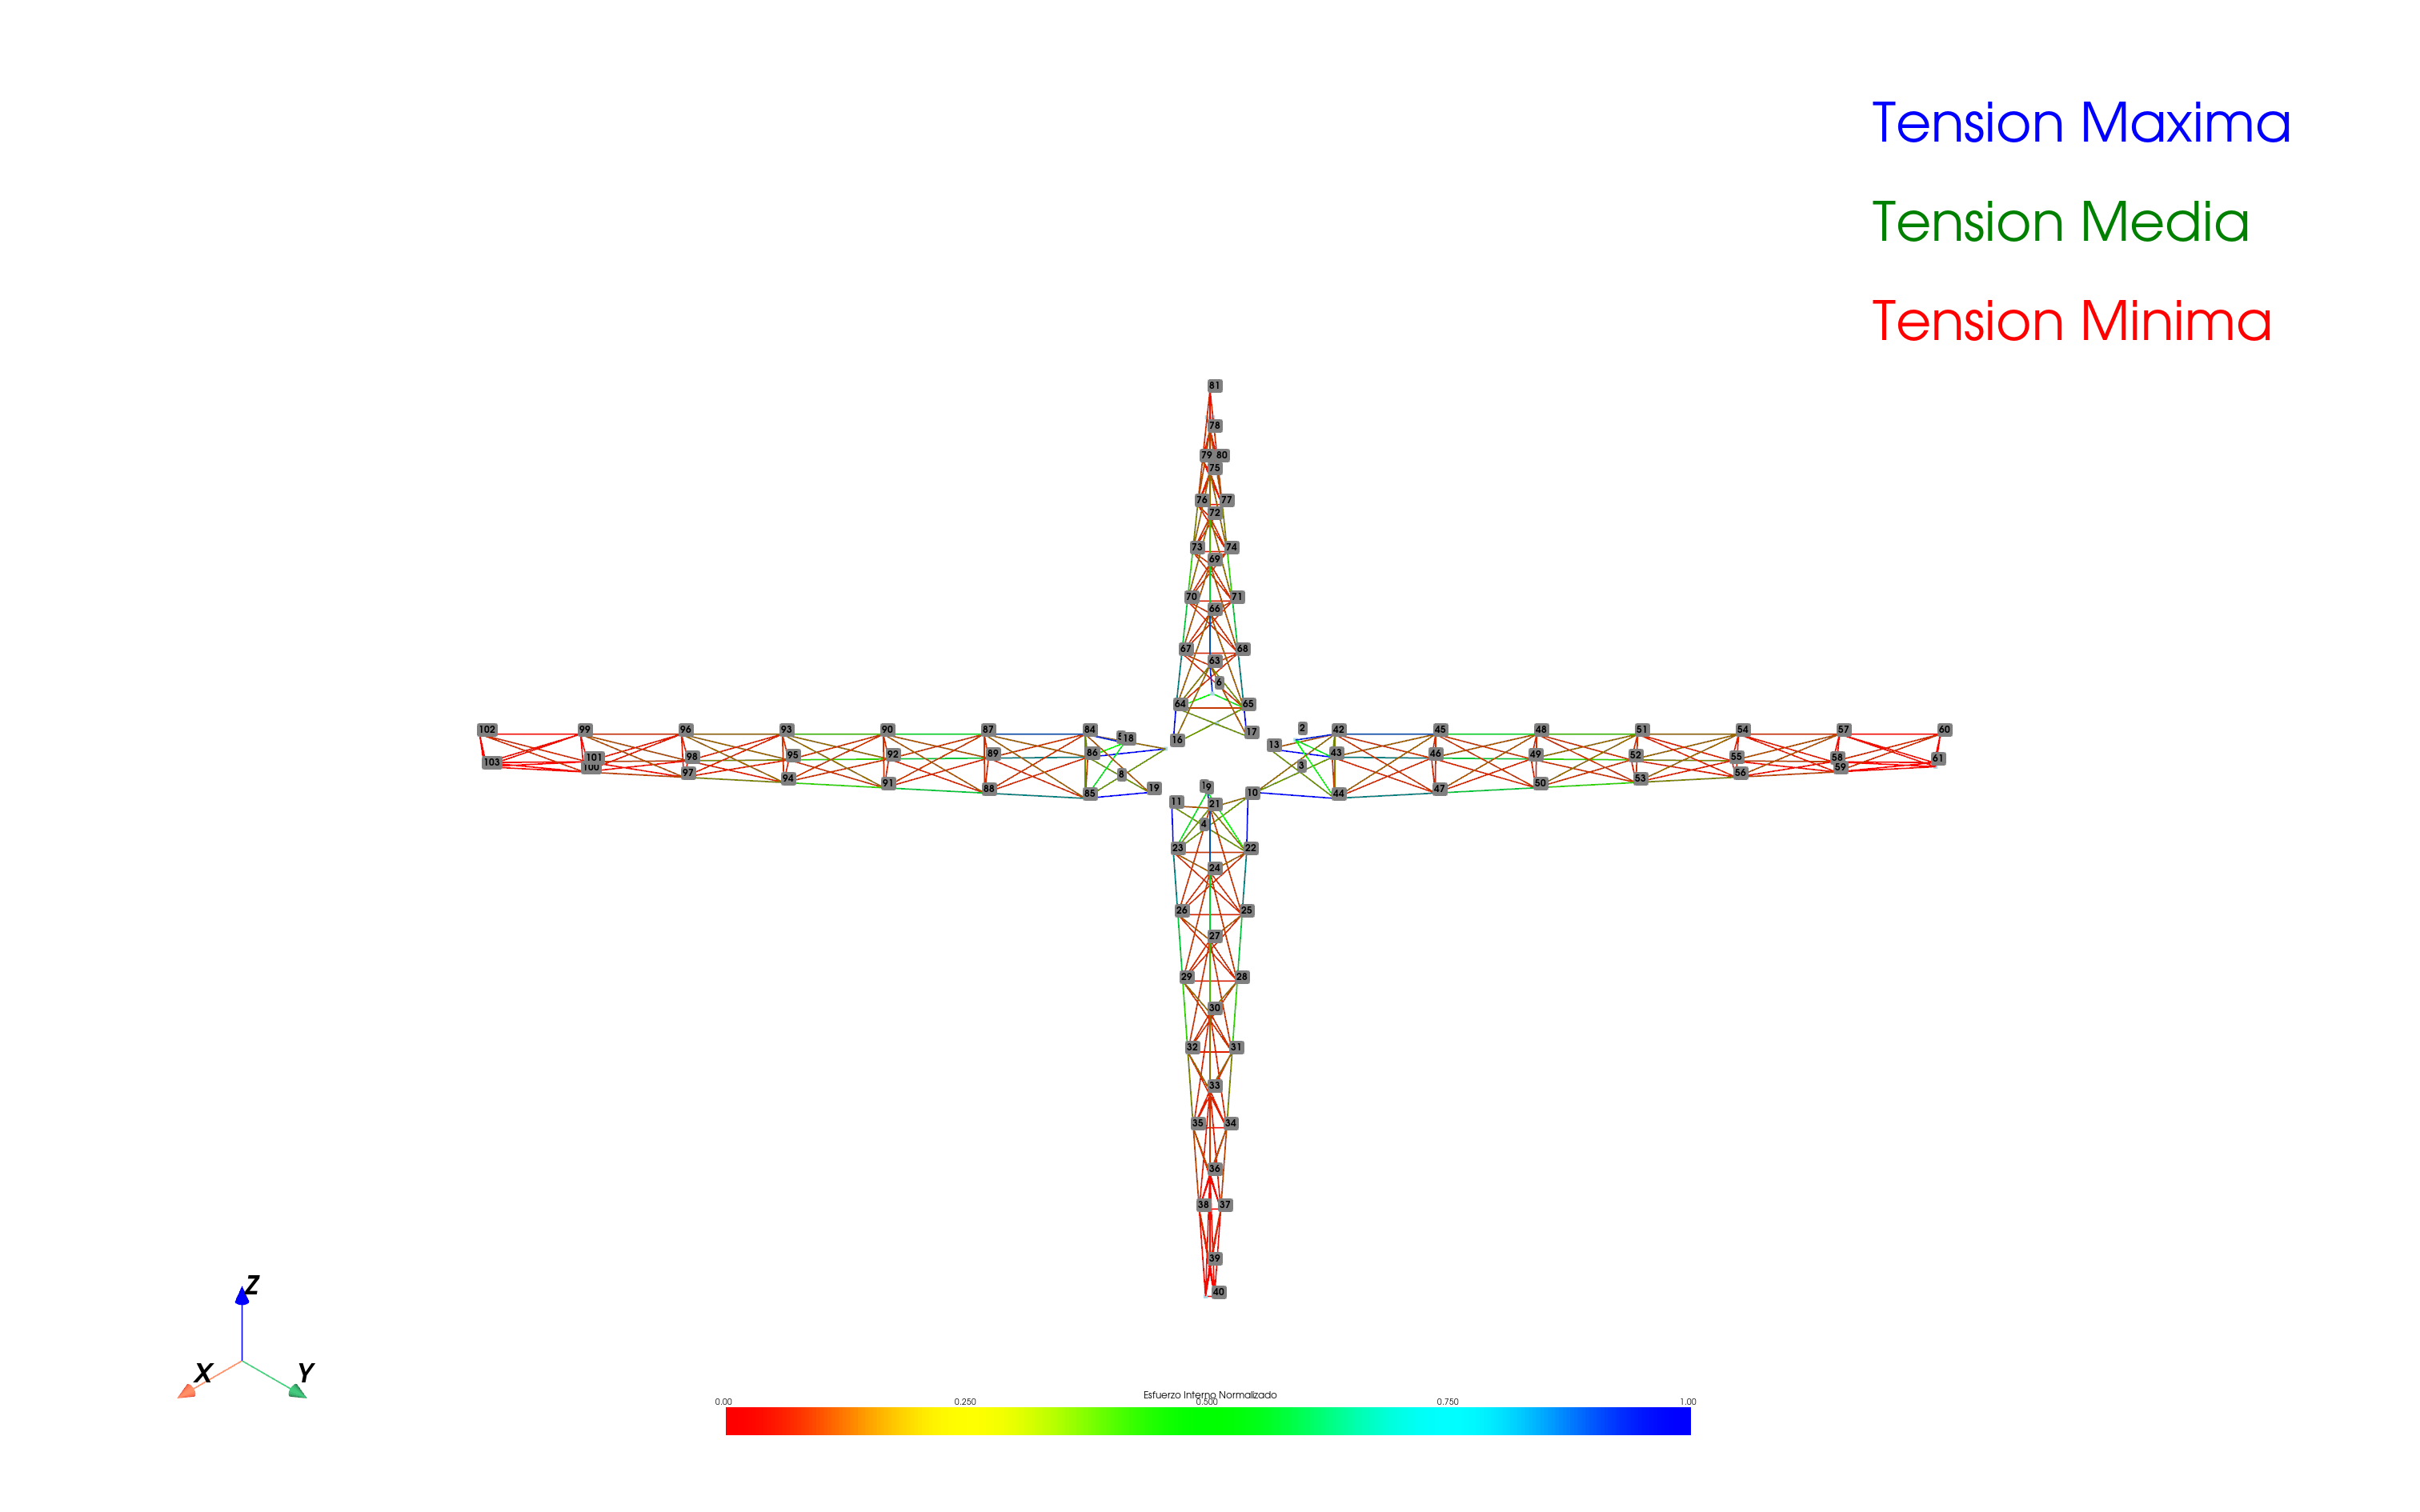
\includegraphics[width=0.8\textwidth]{GRAFICOS_DISENO_LUKAS/esfuerzo_barras_inercia.png}
    \caption{Esfuerzo interno de las barras}
    \label{fig:propuesta1_ei}
\end{figure}

En la Figura \ref{fig:propuesta1_ei}, se observa que el esfuerzo interno de las barras disminuye a medida que se alejan del satélite. Esto ocurre porque las barras más cercanas al satélite soportan la mayor parte de la carga, siendo más afectadas por ella.

\begin{figure}[H]
    \centering
    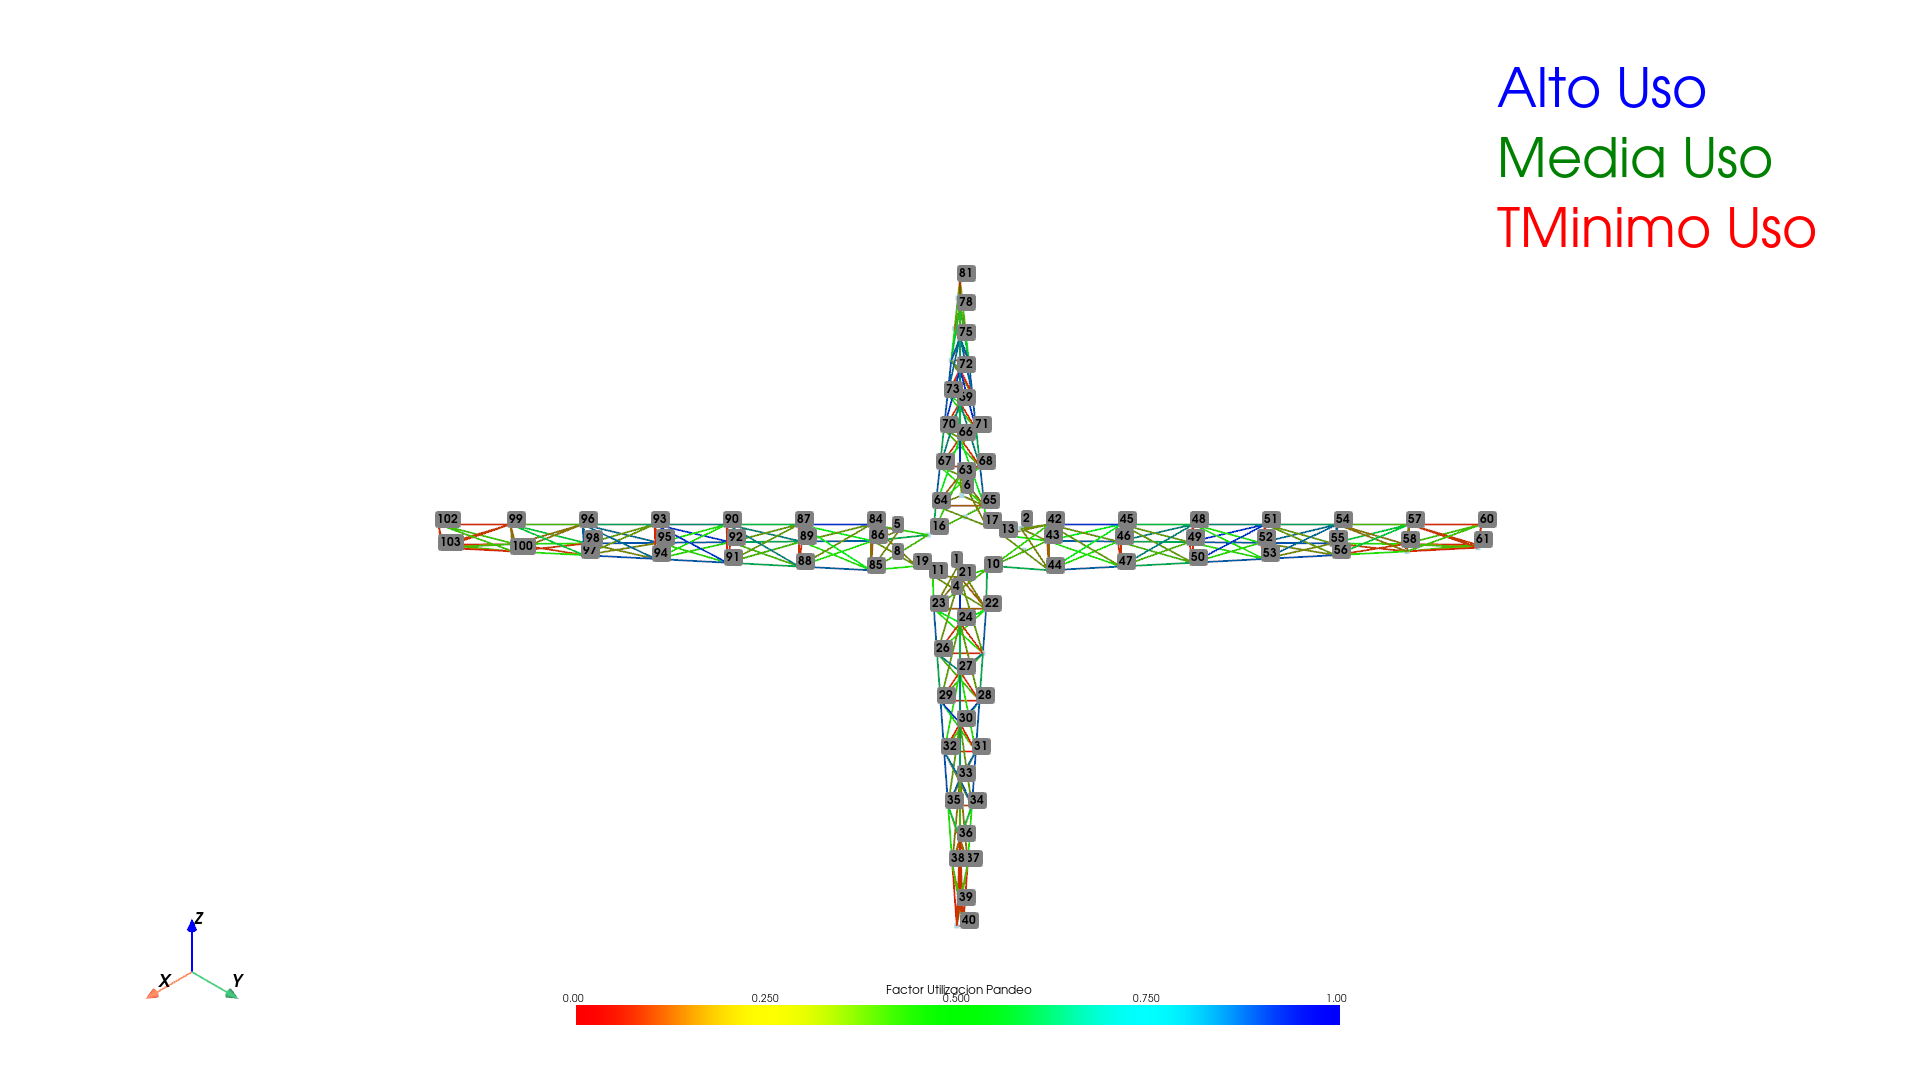
\includegraphics[width=0.8\textwidth]{GRAFICOS_DISENO_LUKAS/factor_utilizacion_pandeo.png}
    \caption{Pandeo de la estructura}
    \label{fig:propuesta1_pandeo}
\end{figure}

En la Figura \ref{fig:propuesta1_pandeo}, se muestra el análisis de pandeo. Este factor es crítico, ya que las barras tienen mayor probabilidad de fallar por este fenómeno. Por ello, se seleccionaron las barras de manera que cumplieran con todos los criterios, considerando un factor de seguridad de 2.

\begin{figure}[H]
    \centering
    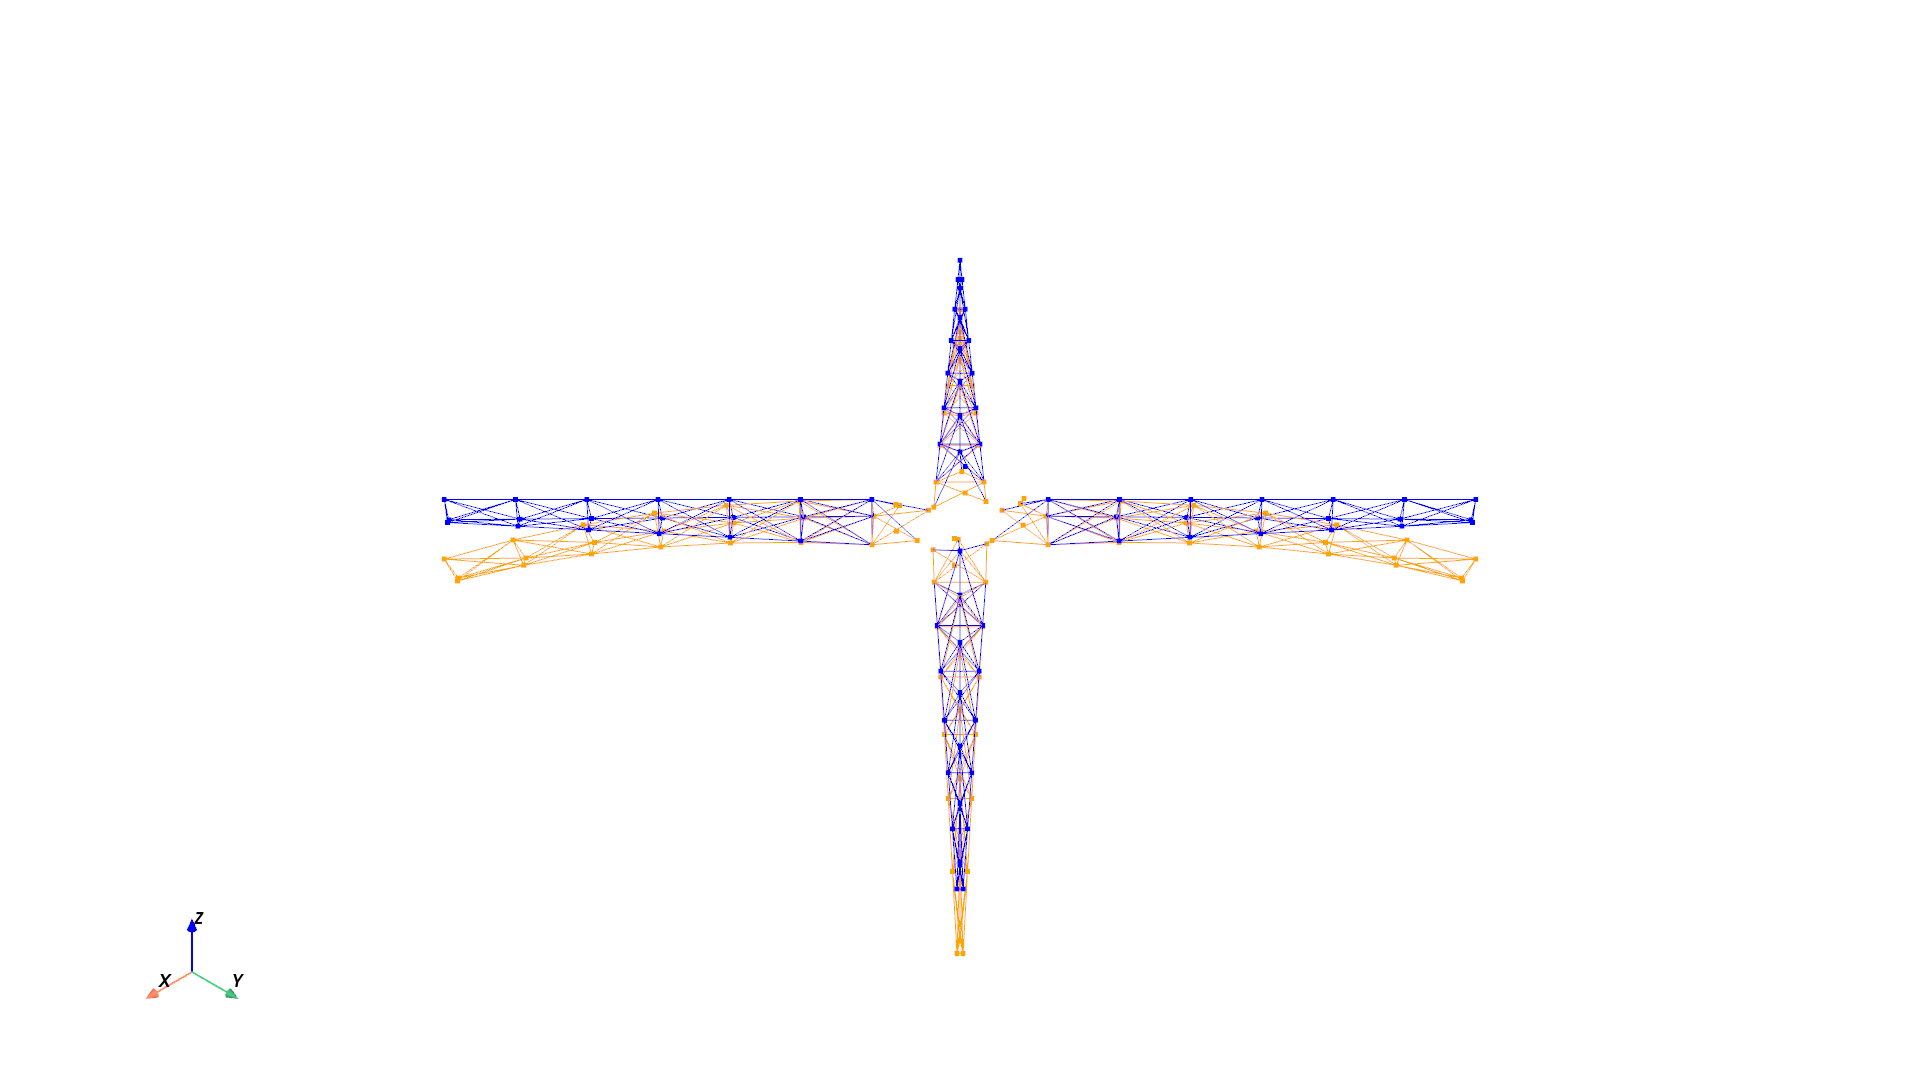
\includegraphics[width=0.8\textwidth]{GRAFICOS_DISENO_LUKAS/desplazamiento_termico.png}
    \caption{Desplazamiento térmico de la estructura}
    \label{fig:propuesta1_termico}
\end{figure}

En la Figura \ref{fig:propuesta1_termico}, se aprecia el desplazamiento térmico. Se asumió que únicamente las barras adyacentes al panel solar son afectadas por el cambio de temperatura, ya que estas reciben el calor de manera directa.

Finalmente, mediante un código denominado \texttt{verificar\_diseño.py} se obtuvieron los siguientes resultados:

\begin{table}[H]
    \centering
    \begin{tabular}{|l|l|c|}
    \hline
    \textbf{Parámetro}              & \textbf{Valor}                     & \textbf{Cumple} \\ \hline
    Masa total barras               & 1161.16 kg                         & -               \\ \hline
    Área total de panel             & 3355.44 m²                         & -               \\ \hline
    Área requerida                  & 3333.33 m²                         & -               \\ \hline
    Suficiente área                 & -                                   & \textbf{True}   \\ \hline
    Masa total panel                & 3690.99 kg                         & -               \\ \hline
    RME                             & 31.46\%                            & -               \\ \hline
    Cumple RME                      & -                                   & \textbf{False}  \\ \hline
    Cumple resistencia              & 0.0 < FU < 0.0182033262645507      & \textbf{True}   \\ \hline
    Cumple pandeo                   & -                                   & \textbf{True}   \\ \hline
    Frecuencia fundamental          & 0.089 Hz                           & \textbf{False}  \\ \hline
    $\theta_\text{all\_max}$        & 0.03208818380943898                & \textbf{True}   \\ \hline
    Cumple $\theta_\text{max}$      & -                                   & \textbf{True}   \\ \hline
    \end{tabular}
    \caption{Resultados de la propuesta número 1 para verificar si el diseño cumple.}
    \label{tabla:modelo_h5_p1}
\end{table}
    
Como se observa, se cumplen casi todos los criterios, excepto el RME y la frecuencia fundamental.

\newpage
\subsection{Propuesta 2}

En este caso, el diseño tiene una forma de H, y se decidió llevar a cabo este diseño ya que se consideró que podía ser un buen punto medio entre la masa de la estructura y su rigidez. Este diseño también se basó en el diseño presentado en \cite{hoyt2014trusselator}, quedando de la siguiente forma:

\begin{figure}[H]
    \centering
    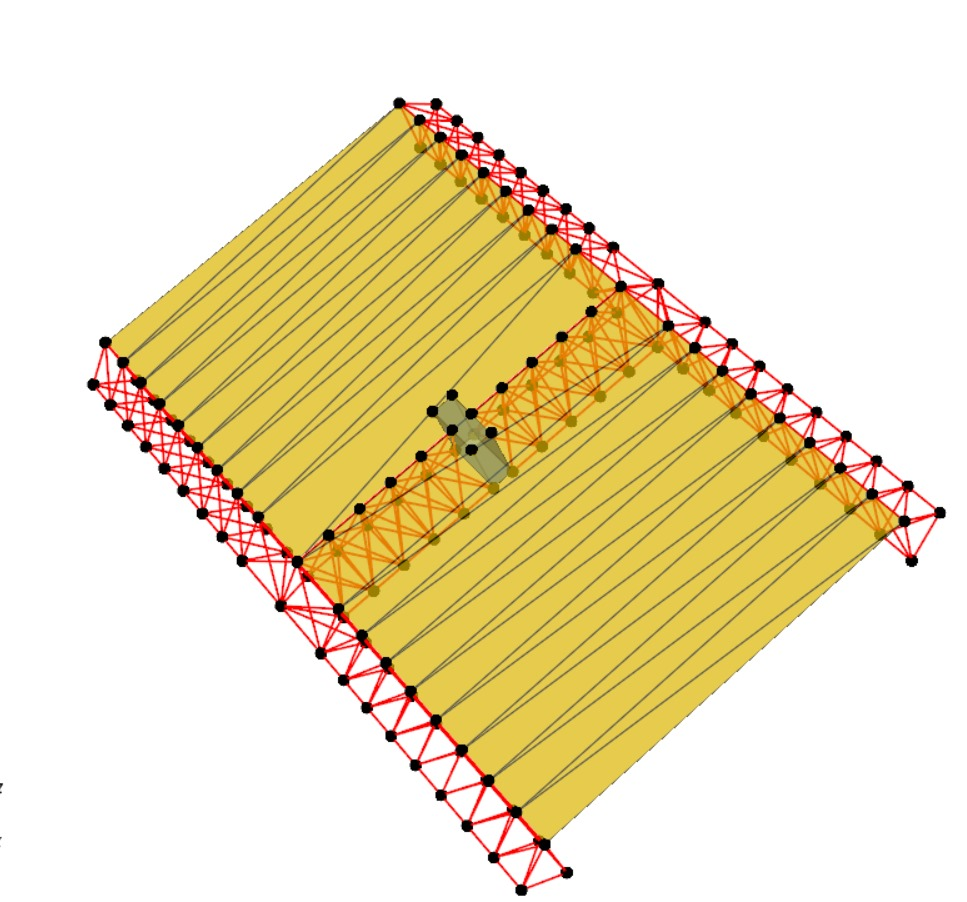
\includegraphics[width=0.8\textwidth]{GRAFICOS_DISENO_BENO/propuesta2.png}
    \caption{Diseño de la propuesta 2 para el satélite}
    \label{fig:propuesta2}
\end{figure}

\subsubsection{Análisis de la estructura}

A continuación, se presentan los resultados de los criterios exigidos para el diseño de la estructura.

\begin{table}[H]
    \centering
    \begin{tabular}{|l|l|c|}
    \hline
    \textbf{Parámetro}              & \textbf{Valor}                     & \textbf{Cumple} \\ \hline
    Cumple soportes                 & -                                   & \textbf{True}   \\ \hline
    Área total de panel             & 3399.48 m²                         & -               \\ \hline
    Área requerida                  & 3333.33 m²                         & -               \\ \hline
    Suficiente área                 & -                                   & \textbf{True}   \\ \hline
    Masa total panel                & 3739.43 kg                         & -               \\ \hline
    Masa total estructura           & 730.26 kg                          & -               \\ \hline
    Inercia total panel             & 736132.10 kg·m²                    & -               \\ \hline
    Inercia total estructura        & 177520.81 kg·m²                    & -               \\ \hline
    RME                             & 19.53\%                            & -               \\ \hline
    Cumple RME                      & -                                   & \textbf{True}   \\ \hline
    Cumple resistencia              & 0.0 < FU < 3.584595626471951e+18   & \textbf{False}  \\ \hline
    Cumple pandeo                   & -                                   & \textbf{True}   \\ \hline
    Frecuencia fundamental          & 0.000 Hz                           & \textbf{Unknown}  \\ \hline
    $\theta_\text{all\_max}$        & 178.06145332574985                 & \textbf{False}  \\ \hline
    Cumple $\theta_\text{max}$      & -                                   & \textbf{False}  \\ \hline
    \end{tabular}
    \caption{Resumen de parámetros del modelo actualizado.}
    \label{tabla:modelo_h5_actualizado}
\end{table}
  
En este analisis se puede apreciar que la propuesta 2 cumple ciertos criterios, aunque no todos. Además, uno de los criterios, que es imporntanrte para el estudio de este diseño, no se da como conocido, que es la frecuencia fundamental.

\subsection{Comparación de propuestas}

Como se puede apreciar en los análisis de las estructuras de las propuestas 1 y 2, la propuesta 1 cumple con una mayor cantidad de criterios de diseño y operación. Además, se consideró que la propuesta 1 es más simple en cuanto a la manipulación de la estructura en el software OpenSeesPy. 

En cuanto a la frecuencia fundamental, la propuesta 1 no cumple con el criterio de diseño, pero se consideró que este diseño es más factible de mejorar para cumplir con este criterio. Por otro lado, la propuesta 2 no cumple con el criterio de resistencia, lo que podría ser un problema más difícil de solucionar, además de que la frecuencia fundamental no se pudo calcular.
\newpage
\section{Propuesta final}

Luego de comparar ambas propuestas, se decidió que la propuesta 1 es la que cumple con una mayor cantidad de requisitos de diseño. Además, se consideró que este diseño tiene una mejor trabajabilidad, por lo que realizarle los cambios necesarios para cumplir completamente con las condiciones de diseño y operación es más factible. Uno de los factores por los cuales se descartó la propuesta 2 es que las deformaciones térmicas son muy grandes, lo que podría afectar el funcionamiento del satélite, además de que cumple con una menor cantidad de condiciones de diseño.

\begin{figure}[H]
    \centering
    \includegraphics[width=0.8\textwidth]{GRAFICOS_DISENO_LUKAS/diseño_satelite.png}
    \caption{Diseño final (Propuesta 1)}
    \label{fig:propuesta1}
\end{figure}

Como se puede apreciar en la tabla \ref{tabla:modelo_h5_p1}, no se cumplen todos los criterios, pero se decidió que este proyecto es más factible y se puede mejorar para que cumpla con todos los requisitos de diseño y operación. El principal objetivo a continuación es que la estructura cumpla con el porcentaje de RME y alcance la frecuencia fundamental esperada. Una vez logrado esto, se podrá optimizar la estructura para que sea lo más eficiente posible.

